% Options for packages loaded elsewhere
\PassOptionsToPackage{unicode}{hyperref}
\PassOptionsToPackage{hyphens}{url}
%
\documentclass[
]{report}
\usepackage{amsmath,amssymb}
\usepackage{iftex}
\ifPDFTeX
  \usepackage[T1]{fontenc}
  \usepackage[utf8]{inputenc}
  \usepackage{textcomp} % provide euro and other symbols
\else % if luatex or xetex
  \usepackage{unicode-math} % this also loads fontspec
  \defaultfontfeatures{Scale=MatchLowercase}
  \defaultfontfeatures[\rmfamily]{Ligatures=TeX,Scale=1}
\fi
\usepackage{lmodern}
\ifPDFTeX\else
  % xetex/luatex font selection
\fi
% Use upquote if available, for straight quotes in verbatim environments
\IfFileExists{upquote.sty}{\usepackage{upquote}}{}
\IfFileExists{microtype.sty}{% use microtype if available
  \usepackage[]{microtype}
  \UseMicrotypeSet[protrusion]{basicmath} % disable protrusion for tt fonts
}{}
\makeatletter
\@ifundefined{KOMAClassName}{% if non-KOMA class
  \IfFileExists{parskip.sty}{%
    \usepackage{parskip}
  }{% else
    \setlength{\parindent}{0pt}
    \setlength{\parskip}{6pt plus 2pt minus 1pt}}
}{% if KOMA class
  \KOMAoptions{parskip=half}}
\makeatother
\usepackage{xcolor}
\usepackage{graphicx}
\makeatletter
\def\maxwidth{\ifdim\Gin@nat@width>\linewidth\linewidth\else\Gin@nat@width\fi}
\def\maxheight{\ifdim\Gin@nat@height>\textheight\textheight\else\Gin@nat@height\fi}
\makeatother
% Scale images if necessary, so that they will not overflow the page
% margins by default, and it is still possible to overwrite the defaults
% using explicit options in \includegraphics[width, height, ...]{}
\setkeys{Gin}{width=\maxwidth,height=\maxheight,keepaspectratio}
% Set default figure placement to htbp
\makeatletter
\def\fps@figure{htbp}
\makeatother
\setlength{\emergencystretch}{3em} % prevent overfull lines
\providecommand{\tightlist}{%
  \setlength{\itemsep}{0pt}\setlength{\parskip}{0pt}}
\setcounter{secnumdepth}{5}
% definitions for citeproc citations
\NewDocumentCommand\citeproctext{}{}
\NewDocumentCommand\citeproc{mm}{%
  \begingroup\def\citeproctext{#2}\cite{#1}\endgroup}
\makeatletter
 % allow citations to break across lines
 \let\@cite@ofmt\@firstofone
 % avoid brackets around text for \cite:
 \def\@biblabel#1{}
 \def\@cite#1#2{{#1\if@tempswa , #2\fi}}
\makeatother
\newlength{\cslhangindent}
\setlength{\cslhangindent}{1.5em}
\newlength{\csllabelwidth}
\setlength{\csllabelwidth}{3em}
\newenvironment{CSLReferences}[2] % #1 hanging-indent, #2 entry-spacing
 {\begin{list}{}{%
  \setlength{\itemindent}{0pt}
  \setlength{\leftmargin}{0pt}
  \setlength{\parsep}{0pt}
  % turn on hanging indent if param 1 is 1
  \ifodd #1
   \setlength{\leftmargin}{\cslhangindent}
   \setlength{\itemindent}{-1\cslhangindent}
  \fi
  % set entry spacing
  \setlength{\itemsep}{#2\baselineskip}}}
 {\end{list}}
\usepackage{calc}
\newcommand{\CSLBlock}[1]{\hfill\break\parbox[t]{\linewidth}{\strut\ignorespaces#1\strut}}
\newcommand{\CSLLeftMargin}[1]{\parbox[t]{\csllabelwidth}{\strut#1\strut}}
\newcommand{\CSLRightInline}[1]{\parbox[t]{\linewidth - \csllabelwidth}{\strut#1\strut}}
\newcommand{\CSLIndent}[1]{\hspace{\cslhangindent}#1}
\usepackage[colorinlistoftodos]{todonotes}
\usepackage{graphicx}
\usepackage{float}
\usepackage{hyperref}
\usepackage{appendix}
\usepackage{caption}
\usepackage{subfigure}
\usepackage{biblatex}
\ifLuaTeX
  \usepackage{selnolig}  % disable illegal ligatures
\fi
\usepackage{bookmark}
\IfFileExists{xurl.sty}{\usepackage{xurl}}{} % add URL line breaks if available
\urlstyle{same}
\hypersetup{
  pdftitle={Time Series Project},
  pdfauthor={Jacob Clinton George Smith-Kolff},
  hidelinks,
  pdfcreator={LaTeX via pandoc}}

\title{Time Series Project}
\author{Jacob Clinton George Smith-Kolff}
\date{2024-10-14}

\begin{document}
\maketitle

{
\setcounter{tocdepth}{1}
\tableofcontents
}
\chapter{Introduction}\label{introduction}

(Probably work on this section last)

\section{What is missing data}\label{what-is-missing-data}

\section{Issues caused by missing
data}\label{issues-caused-by-missing-data}

\section{Structure of the report}\label{structure-of-the-report}

\chapter{Theory}\label{theory}

\section{Time series definition}\label{time-series-definition}

\textbf{Missing at random. This basically means that the missingness in the data is not imformative}

We begin by providing definitions for both uni variate and multivariate
time series:

A univariate time series \(X = \{x_1, x_2, ..., x_t\} \in \mathbb{R}^t\)
is a sequence \(t\) observations on a single variable.\\
This can be extended to multivariate time series:\\
\(X = \{x_1, x_2, ..., x_t\}\in \mathbb{R}^{t\times d}\) where each
\(x_i\) is a \(d\) dimensional vector.

\section{Missing data Mechanisms}\label{missing-data-mechanisms}

Data missingness is a common occurrence that is common in working with
real world data. Missing data can arise from device failures such as
measureing equipment failing, or from data censoring (such as from
governments) {[}1{]}. Missing data typically falls into one of three
categories:

\subsection{Missing Completely at Random
(MCAR)}\label{missing-completely-at-random-mcar}

Data is said to be missing completely at random if the distribution that
describes how missingness occurs is independent of both the observed and
unobserved values in the time series.

\subsection{Missing at Random (MAR)}\label{missing-at-random-mar}

Missing at random is when missingness is related to the observed data,
but is independent of the unobserved data. This means that there is some
external factor that is causing the missingness. An example given in
{[}2{]} is that data from a sensor is more likely to be missing on
weekends since on some weekends the sensor is shutdown.

\subsection{Not Missing at Random
(NMAR)}\label{not-missing-at-random-nmar}

Not missing at random means that the missingness is related to the value
of the observation itself. An example of this is a sensor that will
return a missing value if the recorded value is above 100\(^\circ\).

\todo{Come back and include probability notation}

\section{Missing data imputation}\label{missing-data-imputation}

Most missing data imputation methods require MCAR or MAR, this is
because these systems of missingness are not informative towards the
missing values themselves. \todo[inline]{Can extend this writeup later.}

\todo{Idea is to start with the most basic techniques, then more the more advanced ones}

\subsection{Univariate data
imputation}\label{univariate-data-imputation}

\subsubsection{The struggle with univariate data
imputation}\label{the-struggle-with-univariate-data-imputation}

Unlike with a multivariate time series, a univariate time series is only
one sequence of observations \(\{y_1, y_2, ..., y_n\}\). This simplier
form actually leads to increased difficulty when it comes to imputing a
missing value of \(y\), since we can no longer exploit any dependencies
between the predictor variables in the series. With univariate
imputation we can only rely on the previous (or future) values for \(y\)
along with the implicit time variable \footnote{moritz2015comparison}.

\subsubsection{Last Observed Carried Forward (LOCF) Next Observation
Carried Backward
(NOCB)}\label{last-observed-carried-forward-locf-next-observation-carried-backward-nocb}

\footnote{ahn2022comparison}

\subsubsection{Mean/Median imputation}\label{meanmedian-imputation}

This is another simple approach for filling in a missing value. We take
the mean over the entire series and impute the missing value with the
series mean: \begin{equation}\label{eqn:Mean_imputation}
\hat{\mu} = \sum_i \frac{y_i}{n}
\end{equation}

If we replace Equation \ref{eqn:Mean_imputation} with the median, then
we have median imputation.

\todo[inline]{Keep talking about why this method is not great in general and why it could be worse for series with a trend}

\subsubsection{Spline interpolation}\label{spline-interpolation}

A split interpolation of missing data assumes a linear relationship
between the data points. The equation is given by:
\begin{equation}\label{eqn:Split_interp}
f(x) = f(x_0) + \frac{f(x_1)-f(x_0)}{x_1-x_0}(x_1 - x_0)
\end{equation}

\subsubsection{Kalman filter}\label{kalman-filter}

\subsection{Multivariate data imputation
techniques}\label{multivariate-data-imputation-techniques}

\subsubsection{K-nearest neighbours}\label{k-nearest-neighbours}

K-Nearest neighbours is a simple non-parametric machine learning
algorithm, it can be used for either classification or regression. It
can be applied in a time series data imputation context to estimate
missing values in a time series.

\[\frac{1}{K}\sum_{j=1}^K Y_j\] Consider a missing value \(x_i\) in a
time series, k-nearest neighbours will impute a value for the missing
value by calculating the mean of the data points in the neighbourhood
determined by a distance metric such as Euclidean distance. The
algorithm is simple and is shown to be quite effective {[}3{]}.
K-nearest neighbours algorithm has a hyper-parameter K, the number of
nearest (non missing) data points to consider. A choice of K that is too
large may lead to smoothing over temporal patters (under fitting) this
has the effect of ignoring potentially important seasonal patterns. On
the other hand a value of K that is too small could lead to being overly
sensitive to the noise. The value for K needs to be carefully chosen,
typically by cross validation, but in a time series context it could be
chosen using sliding windows and forward chaining. The curse of
dimensionality is an issue for K-nearest neighbours. With higher
dimension it becomes harder to find data points that are closer, this
can lead to an increased sensitivity to noise and misleading
imputations. The computational cost also increases rapidly with more
dimensions in the data making the algorithm less efficient. Another
issue related to computational cost, K-nearest neighbours is a lazy
learning algorithm so the complete dataset ends up being stored. For
large datasets this can make the algorithm slow, or even infeasible

\todo{Come back to this section later}

\subsubsection{Multivariate Imputation by Chained Equations
(MICE)}\label{multivariate-imputation-by-chained-equations-mice}

MICE is a common imputation technique that is quick to incorporate and
yields effective results. The algorithm begins by using something simple
like mean imputation, to fill in initial missing values.

For each variable where missingness is present, we build a regression
model. From there, lagged values \({y_{t-1}, y_{t-2}...,y_{t-n}}\) as
predictors. This is to say that if \({y(t)}\) is missing. predict using
\(y_{t-1}\) and other variables.

impute the missing values for one variable at a time. After that
variable is imputed, use the updated data and move on to the next
variable. We repeat this process until we reach convergence for our
given variable.

This chained process is typically repeated 5-10 times to generate
multiple datasets that contain a variation of results.

After, each data set that has undergone imputation is analysed. Then, we
combine the results using Rubin's rule.

Rubin's rule is as follows:

\begin{enumerate}
\def\labelenumi{\arabic{enumi}.}
\item
  \textbf{Pooled Estimate} (e.g., mean, regression coefficient):

  \[\hat{\theta} = \frac{1}{m}\sum_{i=1}^{m}\theta_{i}\]
\end{enumerate}

where \(\hat{\theta}\) is the pooled estimate, \(m\) is the number of
imputed datasets, and \(\theta_i\) is the estimate in each imputed
dataset \(i\).

\subsubsection{General Adversarial Networks
(GANs)}\label{general-adversarial-networks-gans}

GANs consist of two neural networks. A generator \((G)\), and a
discriminator \((D)\) . These two networks are trained simultaneously
through a game theory approach. It is the generators job to try and
generate realistic data points, while the discriminator tries to
distinguish whether the values are true values or values generated from
the generator. The generator is tasked to try and fool the
discriminator. In turn, attempting to learn the underlying distribution
of the data. This class of machine learning models were first purposed
in 2014 {[}4{]}.

The typical process of using a GAN is as follows:

\begin{enumerate}
\def\labelenumi{\arabic{enumi})}
\item
  The generator produces an estimate for the missing values conditioned
  on \textbf{all} available observed data points.
\item
  The discriminator evaluates the quality of the imputed value compared
  to real observed values.
\item
  Both networks are trained to improve the generators ability to fool
  the discriminator.
\end{enumerate}

The training process continues until the generator can emulate realistic
data that will fool the discriminator and in turn, replicate the
distribution of the observed data. Given this, GANs can provide a
powerful architecture for imputing missing values. Particularly in cases
where imputing techniques can struggle to model the complex
relationships within the data {[}4{]}.

\begin{figure}[h]
\centering
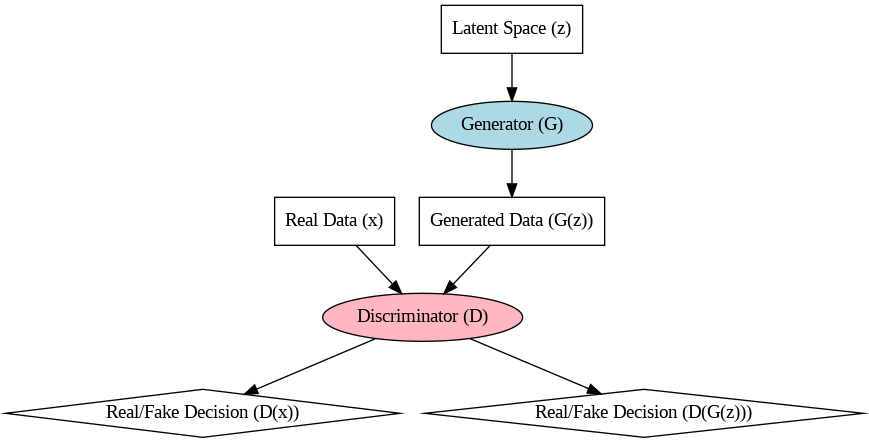
\includegraphics[width=\textwidth]{graphs/gan_architecture.png}


\caption{Structure of our GAN for TS imputation}
\label{fig:Structure_of_gan}  % Corrected spelling
\end{figure}

In our GAN, we use a standard Generator \((G)\)and Discriminator \((D)\)
to handle missing value imputation. The generator receives a sampled
vector from the latent space \((Z)\) and uses that to estimate missing
data points. The discriminator then evaluates whether the generated data
follows the true observed data. Trained using a minimax game where the
generator tries to keep fooling the discriminator.

\chapter{Illustration of time series
imputation}\label{illustration-of-time-series-imputation}

\begin{figure}[ht]
  \centering
  \subfigure[Data imputation on Sunspots]{
    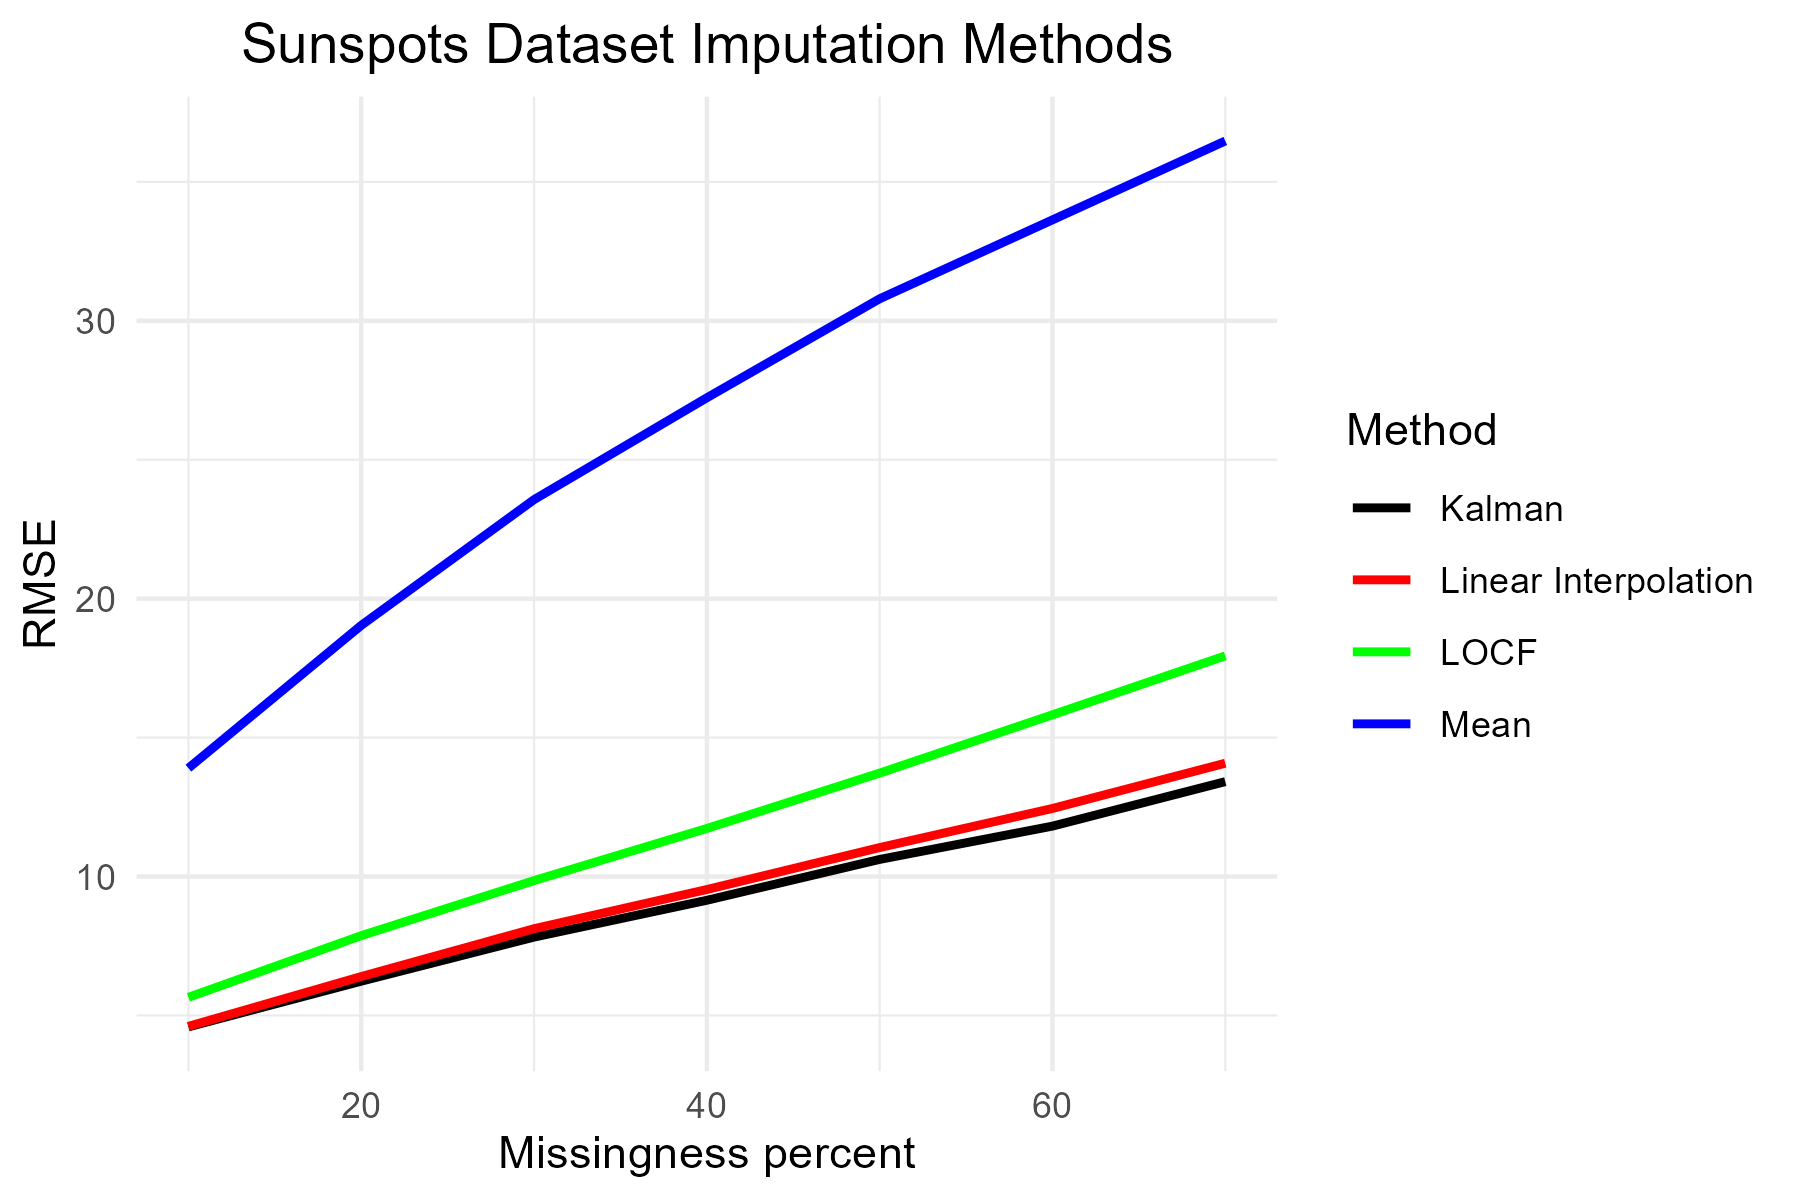
\includegraphics[width=0.45\textwidth]{graphs/univariate/sunspots.png}
    \label{fig:sunspots}
  }
  \subfigure[Data imputation on LakeHeuron]{
    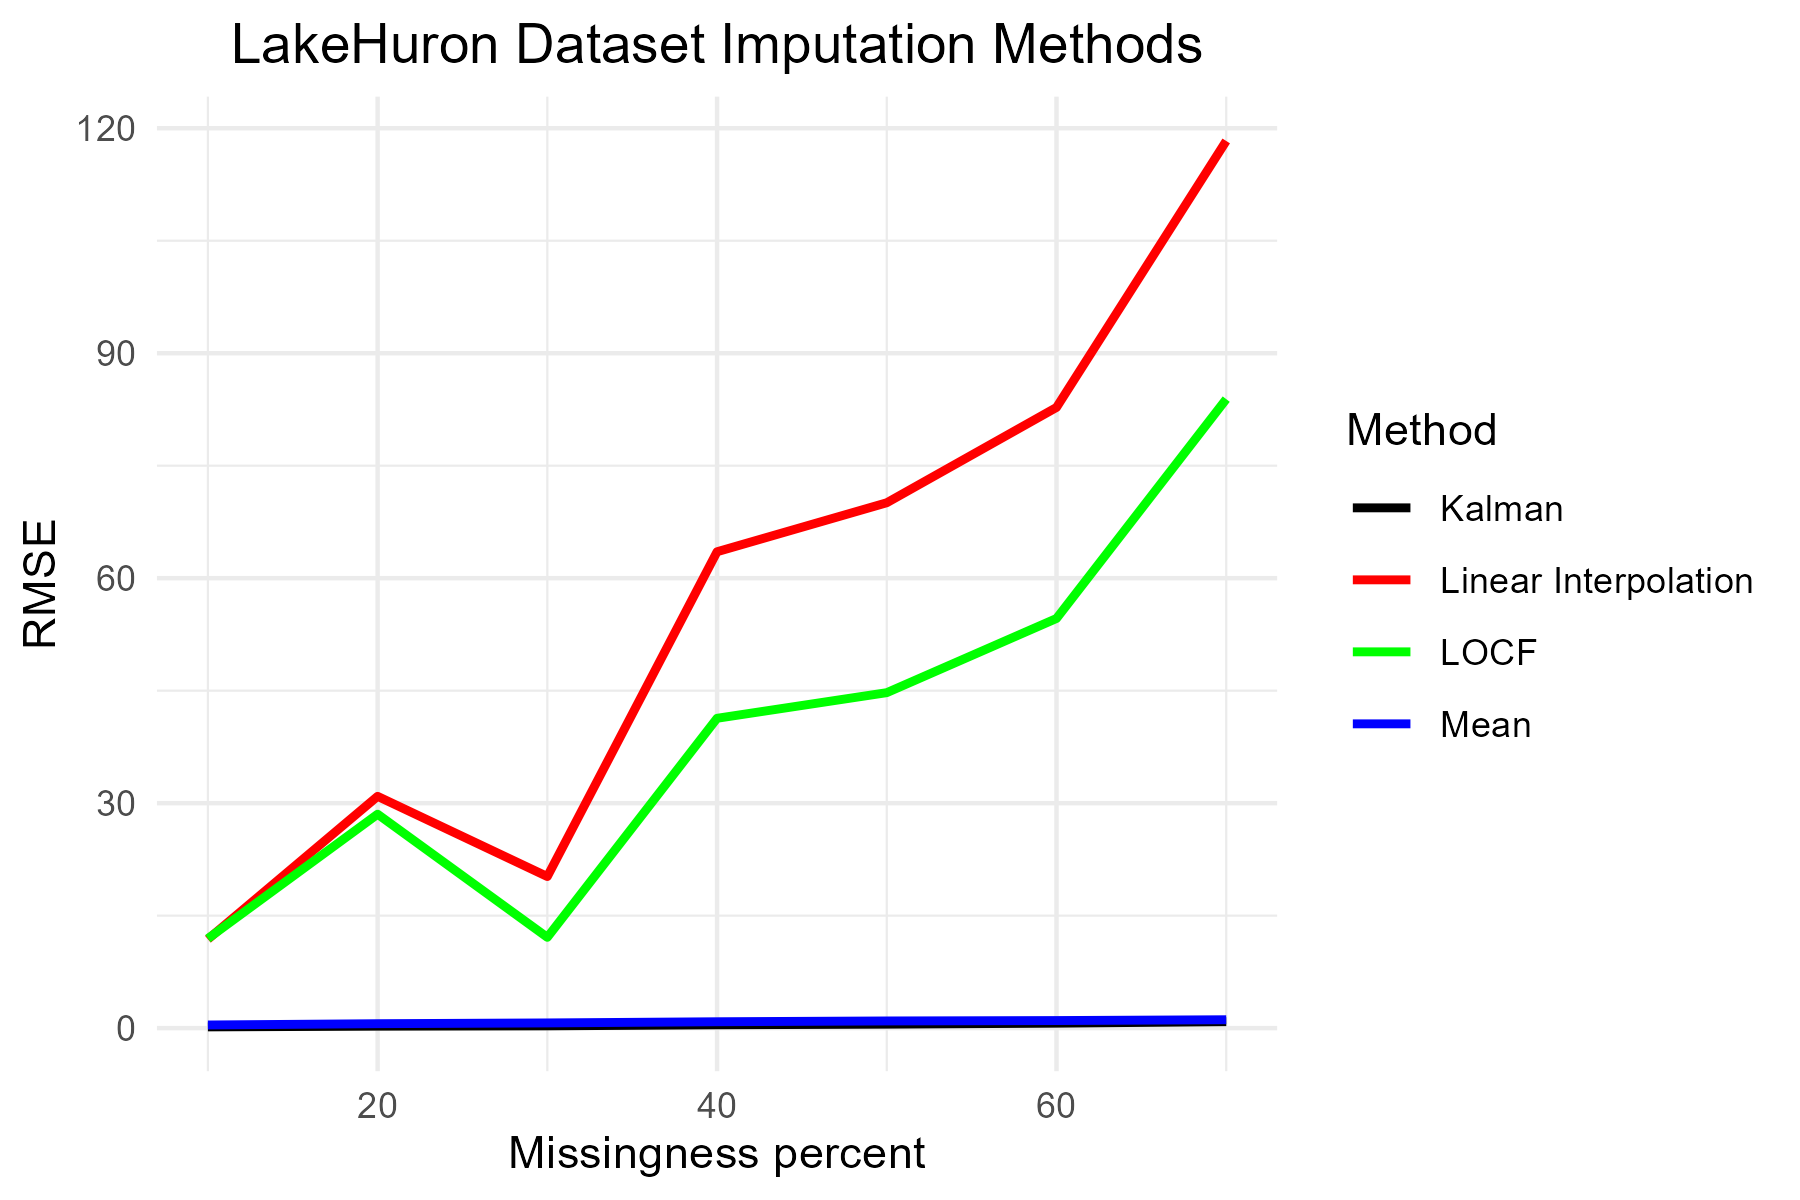
\includegraphics[width=0.45\textwidth]{graphs/univariate/lake.png}
    \label{fig:lake}
  }
  \subfigure[Data imputation on BeerSales]{
    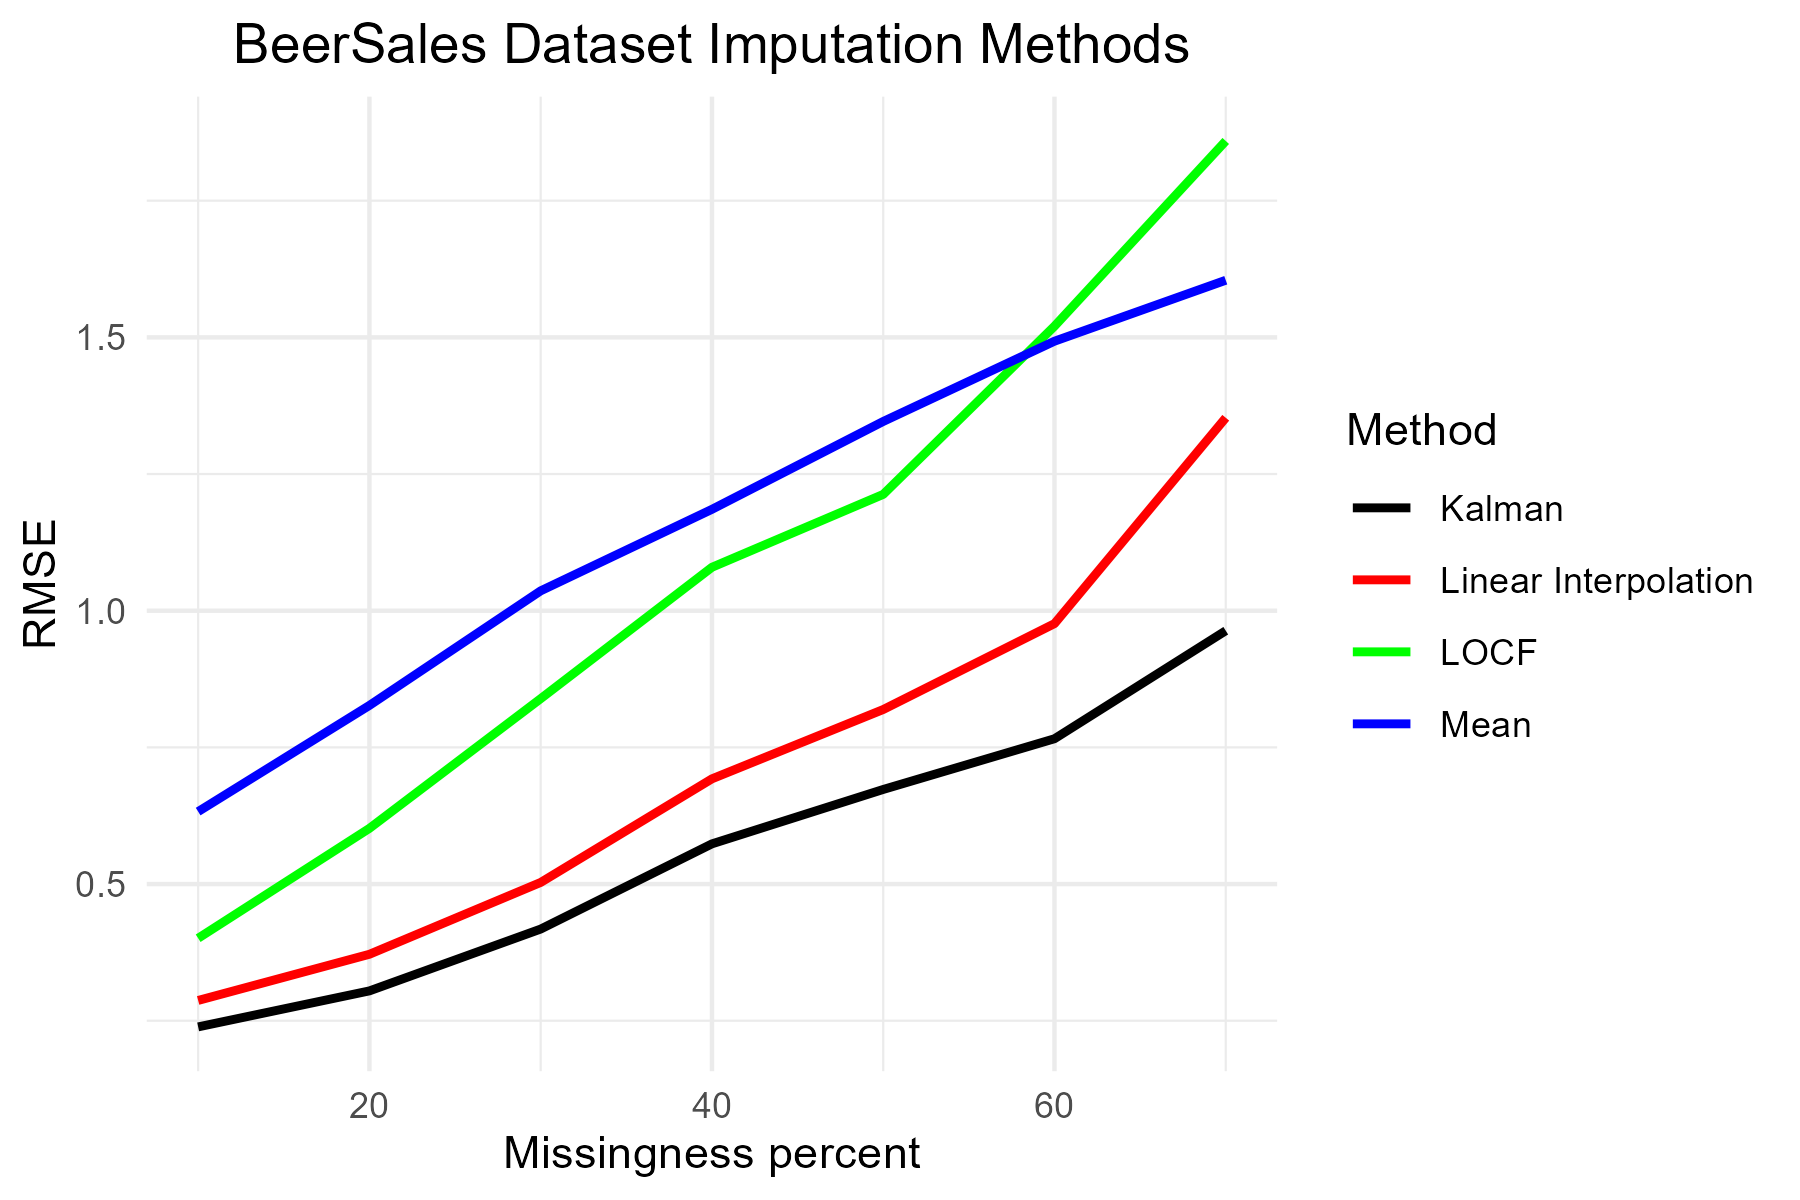
\includegraphics[width=0.45\textwidth]{graphs/univariate/beer.png}
    \label{fig:beer}
  }
  \subfigure[Data imputation on Lynx]{
    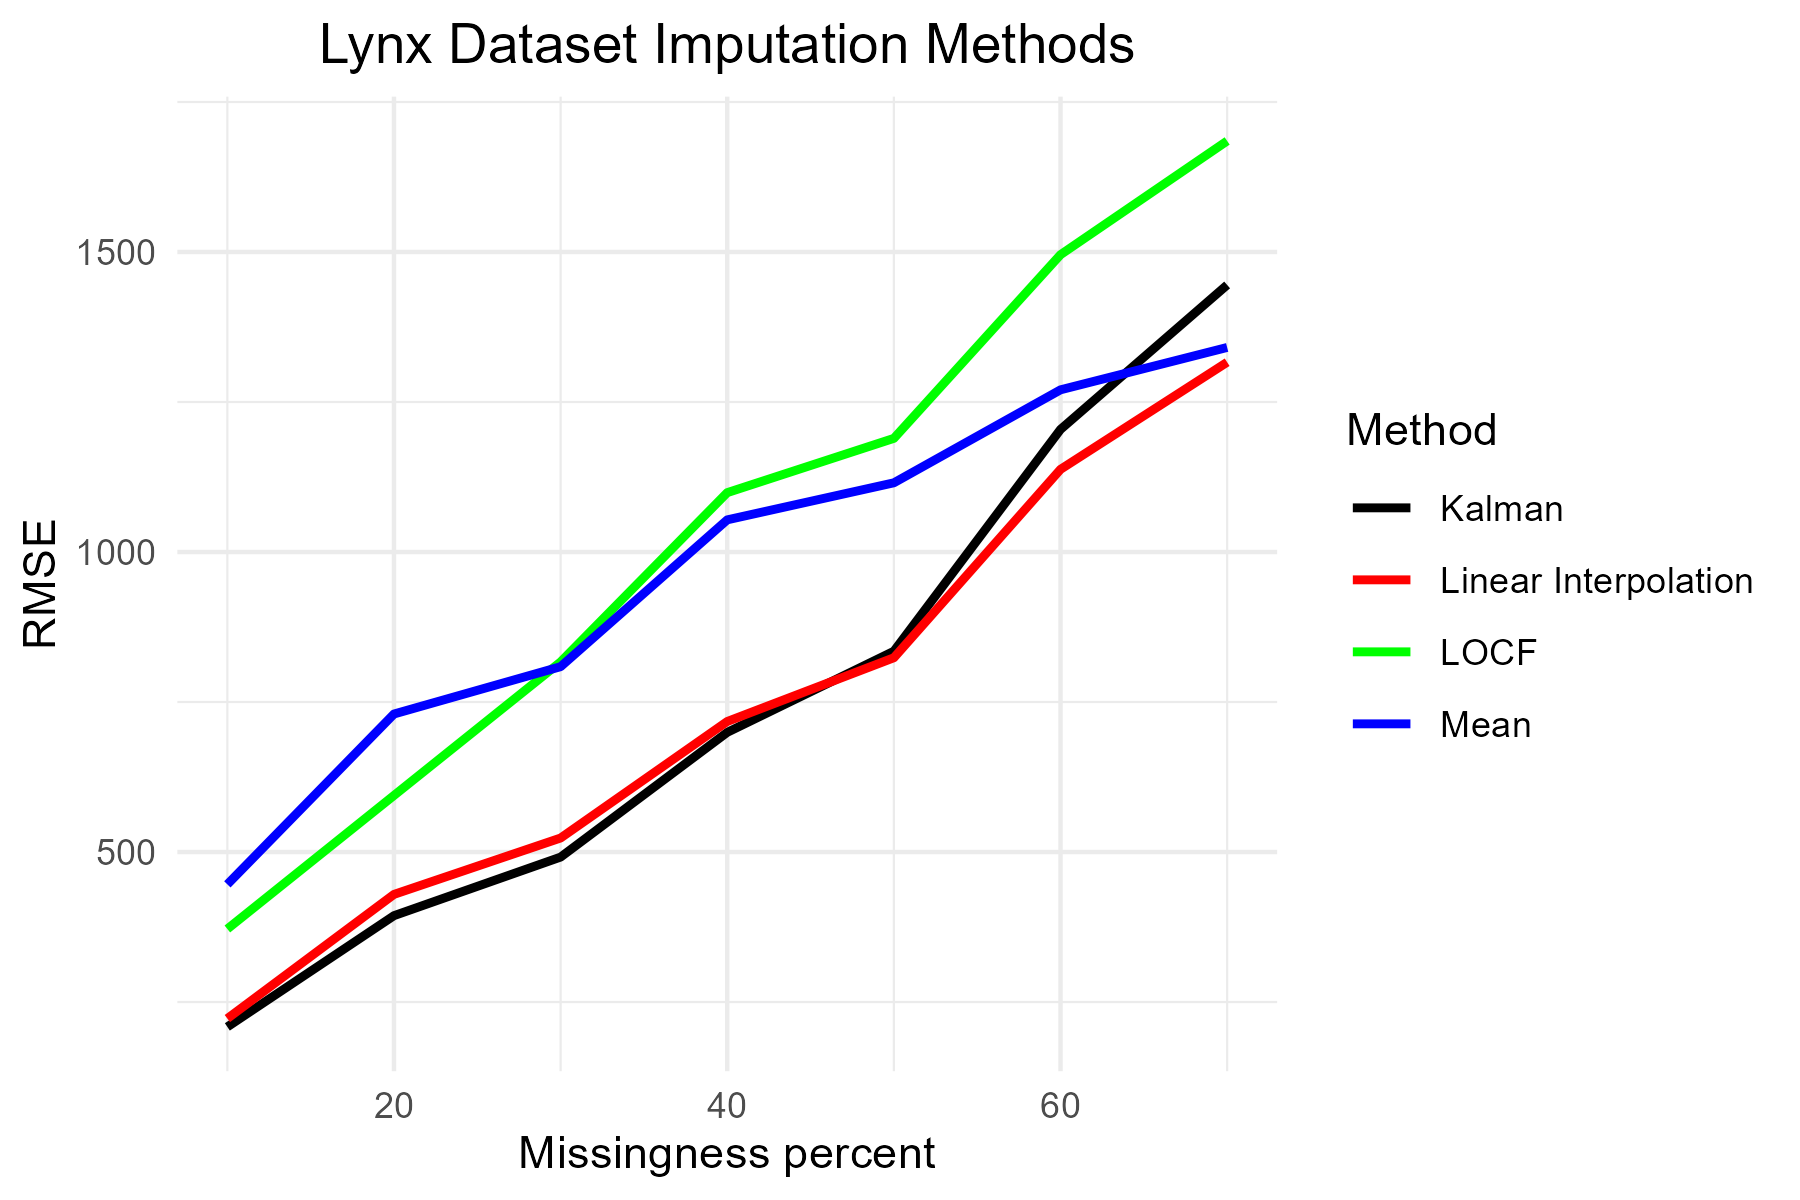
\includegraphics[width=0.45\textwidth]{graphs/univariate/lynx.png}
    \label{fig:lynx}
  }
  \caption{Comparison of Locf, Mean, Linear, and Kalman data inputation on four datasets}
  \label{fig:Univarite_comparison}
\end{figure}

\chapter{Discussion}\label{discussion}

\printbibliography

\chapter*{Appendix}\label{appendix}
\addcontentsline{toc}{chapter}{Appendix}

\phantomsection\label{refs}
\begin{CSLReferences}{0}{0}
\bibitem[\citeproctext]{ref-little2019statistical}
\CSLLeftMargin{{[}1{]} }%
\CSLRightInline{R. J. Little and D. B. Rubin, \emph{Statistical analysis
with missing data}, vol. 793. John Wiley \& Sons, 2019.}

\bibitem[\citeproctext]{ref-moritz2015comparison}
\CSLLeftMargin{{[}2{]} }%
\CSLRightInline{S. Moritz, A. Sardá, T. Bartz-Beielstein, M. Zaefferer,
and J. Stork, {``Comparison of different methods for univariate time
series imputation in r,''} \emph{arXiv preprint arXiv:1510.03924},
2015.}

\bibitem[\citeproctext]{ref-ahn2022comparison}
\CSLLeftMargin{{[}3{]} }%
\CSLRightInline{H. Ahn, K. Sun, K. P. Kim, \emph{et al.}, {``Comparison
of missing data imputation methods in time series forecasting,''}
\emph{Computers, Materials \& Continua}, vol. 70, no. 1, pp. 767--779,
2022.}

\bibitem[\citeproctext]{ref-NIPS2014_5ca3e9b1}
\CSLLeftMargin{{[}4{]} }%
\CSLRightInline{I. Goodfellow \emph{et al.}, {``Generative adversarial
nets,''} in \emph{Advances in neural information processing systems}, Z.
Ghahramani, M. Welling, C. Cortes, N. Lawrence, and K. Q. Weinberger,
Eds., Curran Associates, Inc., 2014. Available:
\url{https://proceedings.neurips.cc/paper_files/paper/2014/file/5ca3e9b122f61f8f06494c97b1afccf3-Paper.pdf}}

\end{CSLReferences}

\end{document}
